\documentclass{article}

\usepackage{polski}
\usepackage[utf8]{inputenc}
\usepackage{graphicx}
\usepackage{float}
\usepackage[margin=1in]{geometry}
\usepackage{graphicx}
\usepackage{amsmath}
\usepackage{mathtools}
\usepackage{amssymb}
\usepackage{multirow}
\usepackage{changepage}
\usepackage{pbox}
\usepackage{indentfirst}
\usepackage{booktabs}

\title{Sprawozdanie}
\begin{document}

\newcommand{\unit}[1]{\thinspace \mathrm{#1}}
	
\begin{center}
	\bgroup
	\def\arraystretch{1.5}
	\begin{tabular}{|c|c|c|c|c|c|}
		\hline
		EAIiIB & \multicolumn{2}{|c|}{\begin{tabular}{@{}c@{}} Tymoteusz Paszun\\ Piotr Morawiecki\end{tabular}} & Rok II & Grupa 3a & Zespół 6 \\
		\hline
		\multicolumn{3}{|c|}{\begin{tabular}{c}Temat: \\ Współczynnik załamania ciał stałych \end{tabular}} & 
		\multicolumn{3}{|c|}{\begin{tabular}{c}Numer ćwiczenia: \\ 51 \end{tabular}} \\
		\hline
		{\begin{tabular}{@{}c@{}} Data wykonania\\ 18.10.2017\end{tabular}}&{\begin{tabular}{@{}c@{}} Data oddania\\ 24.10.2017\end{tabular}}& Zwrot do poprawki & Data oddania & Data zaliczenia & Ocena \\[8ex]
		\hline
	\end{tabular}
	\egroup
\end{center}  

	%WSTEP
\section{Cel ćwiczenia}
Wyznaczenie współczynnika załamania światła dla ciał stałych metodą mikroskopu. 
Zbadanie zależności współczynnika załamania od długości fali.
\section{Wstęp teoretyczny}
Gdy wiązka światła przechodzi przez dwa ośrodki o różnych własnościach optycznych, to na powierzchni granicznej częściowo zostaje odbita, częściowo zaś przechodzi do drugiego środowiska, ulegając załamaniu.
Prawo załamania:
$$\frac{sin \alpha}{sin \beta} = n$$ 
Wielkość $n$ jest stała zwaną współczynnikiem załamania ośrodka drugiego względem ośrodka pierwszego. Współczynnik załamania zależy od długości fali światła padającego. 
\begin{figure}[!htb]
	\centering
	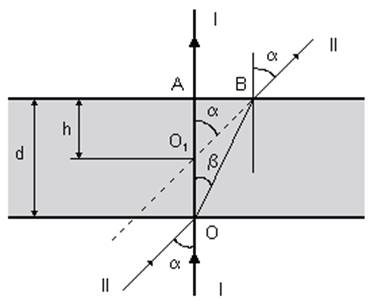
\includegraphics[width=90mm]{image006.jpg}
	\caption{Powstanie pozornego obrazu $O_{1}$ punktu $O$ leżącego na dolnej  powierzchni płytki płaskorównoległej }
\end{figure}

\clearpage
\section{Układ pomiarowy}
W skład układu pomiarowego wchodzą: 
\begin{enumerate}
\item Mikroskop wyposażony w czujnik mikrometryczny i nasadkę krzyżową.
\item Śruba mikrometryczna. 
\item Zestaw płytek szklanych i z pleksiglasu, różnej grubości.
\item Kolorowe filtry.
\end{enumerate}
\section{Wyniki pomiarów}

	\begin{adjustwidth}{-1cm}{}
\def\arraystretch{1.3}

\begin{center}
	\begin{tabular}{|c|c|c|c|c|}
		\hline
		\multicolumn{5}{|l|}{\begin{tabular}{l} Materiał: szkło\\ Grubość rzeczywista: $d = 5,34 \unit{[mm]}$\\ niepewność $u(d) = 0,01 \unit{[mm]}$ \end{tabular}}\\
		\hline
		\multirow{3}{*}{Lp.} & \multicolumn{2}{|c|}{Wskazanie czujnika} & \begin{tabular}{c}Grubość \\pozorna\end{tabular} &\begin{tabular}{c}Współczynnik \\załamania\end{tabular} \\ \cline{2-5}
		& \parbox[c]{1.8 cm}{\centering $a_{d}$}  & $a_{g}$ & $h=a_{d}-a_{g}$ & \multirow{2}{*}{$n=\frac{d}{h}$}\\ \cline{2-4}
		& [mm] & [mm] & [mm] & \\ 
		
		\hline
		1. & 7,40 & 4,26& 3,14& 1,701\\
		\hline
		2. &  7,42& 4,30& 3,12& 1,712\\
		\hline
		3. & 7,47 & 4,36& 3,11& 1,717\\
		\hline
		4. & 7,44 & 4,37& 3,07& 1,739\\
		\hline
		5. & 7,42 & 4,39& 3,03& 1,762\\
		\hline
		6. & 7,50 & 4,31& 3,19& 1,674\\
		\hline
		7. & 7,42 & 4,36& 3,06& 1,745\\
		\hline
		8. & 7,45 & 4,37& 3,08& 1,734\\
		\hline
		\multicolumn{2}{c|}{}&\begin{tabular}{c}Wartość \\ średnia \end{tabular}&3,10 &1,723 \\
		\cline{3-5}
		\multicolumn{2}{c|}{}&\begin{tabular}{c}Niepewność \end{tabular}& 0,018& 0,0104\\
		\cline{3-5}
	\end{tabular}
	\end{center}
\end{adjustwidth}

	\begin{adjustwidth}{-1cm}{}
	\def\arraystretch{1.3}
	
	\begin{center}
		\begin{tabular}{|c|c|c|c|c|}
			\hline
			\multicolumn{5}{|l|}{\begin{tabular}{l} Materiał: szkło\\ Grubość rzeczywista: $d = 2,97 \unit{[mm]}$\\ niepewność $u(d) = 0,01 \unit{[mm]}$ \end{tabular}}\\
			\hline
			\multirow{3}{*}{Lp.} & \multicolumn{2}{|c|}{Wskazanie czujnika} & \begin{tabular}{c}Grubość \\pozorna\end{tabular} &\begin{tabular}{c}Współczynnik \\załamania\end{tabular} \\ \cline{2-5}
			& \parbox[c]{1.8 cm}{\centering $a_{d}$}  & $a_{g}$ & $h=a_{d}-a_{g}$ & \multirow{2}{*}{$n=\frac{d}{h}$}\\ \cline{2-4}
			& [mm] & [mm] & [mm] & \\ 
			
			\hline
			1. & 8,10 & 6,18& 1,92& 1,547\\
			\hline
			2. &  8,08& 6,21& 1,87& 1,588\\
			\hline
			3. & 8,04 & 6,19& 1,85& 1,605\\
			\hline
			4. & 8,09 & 6,19& 1,90& 1,563\\
			\hline
			5. & 8,13 & 6,18& 1,94& 1,523\\
			\hline
			6. & 8,08 & 6,19& 1,89& 1,571\\
			\hline
			7. & 8,09 & 6,16& 1,93& 1,539\\
			\hline
			8. & 8,09 & 6,19& 1,90& 1,563\\
			\hline
			\multicolumn{2}{c|}{}&\begin{tabular}{c}Wartość \\ średnia \end{tabular}&1,90 &1,562 \\
			\cline{3-5}
			\multicolumn{2}{c|}{}&\begin{tabular}{c}Niepewność \end{tabular}& 0,011& 0,0108\\
			\cline{3-5}
		\end{tabular}
	\end{center}
\end{adjustwidth}

	\begin{adjustwidth}{-1cm}{}
	\def\arraystretch{1.3}
	
	\begin{center}
		\begin{tabular}{|c|c|c|c|c|}
			\hline
			\multicolumn{5}{|l|}{\begin{tabular}{l} Materiał: pleksiglas\\ Grubość rzeczywista: $d = 3,88 \unit{[mm]}$\\ niepewność $u(d) = 0,01 \unit{[mm]}$ \end{tabular}}\\
			\hline
			\multirow{3}{*}{Lp.} & \multicolumn{2}{|c|}{Wskazanie czujnika} & \begin{tabular}{c}Grubość \\pozorna\end{tabular} &\begin{tabular}{c}Współczynnik \\załamania\end{tabular} \\ \cline{2-5}
			& \parbox[c]{1.8 cm}{\centering $a_{d}$}  & $a_{g}$ & $h=a_{d}-a_{g}$ & \multirow{2}{*}{$n=\frac{d}{h}$}\\ \cline{2-4}
			& [mm] & [mm] & [mm] & \\ 
			
			\hline
			1. & 7,81 & 5,34& 2,47& 1,571\\
			\hline
			2. &  7,86& 5,30& 2,56& 1,516\\
			\hline
			3. & 7,845 & 5,35& 2,495& 1,555\\
			\hline
			4. & 7,85 & 5,33& 2,52& 1,540\\
			\hline
			5. & 7,85 & 5,35& 2,50& 1,552\\
			\hline
			6. & 7,845 & 5,34& 2,51& 1,549\\
			\hline
			7. & 7,83 & 5,33& 2,50& 1,552\\
			\hline
			8. & 7,835 & 5,33& 2,51& 1,549\\
			\hline
			\multicolumn{2}{c|}{}&\begin{tabular}{c}Wartość \\ średnia \end{tabular}&2,51 &1,548 \\
			\cline{3-5}
			\multicolumn{2}{c|}{}&\begin{tabular}{c}Niepewność \end{tabular}& 0,009& 0,0069\\
			\cline{3-5}
		\end{tabular}
	\end{center}
\end{adjustwidth}

\begin{adjustwidth}{-1cm}{}
	\def\arraystretch{1.3}
	\begin{center}
	\begin{tabular}{|c|c|c|c|c|c|c|}
		\hline
		\multicolumn{4}{|l|}{Materiał: pleksiglas} & \multicolumn{3}{|l|}{Grubość rzeczywista $d$=3,88[mm]}\\
		\hline
		\multicolumn{2}{|c|}{\parbox[c]{2.4cm}{\centering Długość fali}} & \multicolumn{2}{|c|}{Wskazanie czujnika} & \begin{tabular}{c}Grubość \\pozorna\end{tabular} &\begin{tabular}{@{}c@{}}Współczynnik \\załamania\end{tabular} & \begin{tabular}{c}Wartość \\średnia\end{tabular} \\ 
		\hline
		\multicolumn{2}{|c|}{$\lambda$} & \parbox[c]{1.4cm}{\centering $a_{d}$}  & $a_{g}$ & $h=a_{d}-a_{g}$ & \multirow{2}{*}{$n=\frac{d}{h}$} & \multirow{2}{*}{$n_{sr}$} \\ 
		\cline{1-5}
		\multicolumn{2}{|c|}{[$\mu m$]} & [mm] &[mm] &[mm] & & \\ 
		\hline
				\multirow{5}{*}{I} & \multirow{5}{*}{\parbox[c]{1cm}{Niebieski 0,48}} & 7,78& 5,24& 2,54& 1,528& \multirow{5}{*}{1,522} \\
				\cline{3-6}
				& & 7,80& 5,245& 2,555& 1,519& \\
				\cline{3-6}
				& & 7,84& 5,25& 2,59& 1,498& \\
				\cline{3-6}
				& & 7,78& 5,24& 2,54& 1,528& \\
				\cline{3-6}
				& & 7,80& 5,25& 2,55& 1,522& \\
				\hline
		\multirow{5}{*}{II} & \multirow{5}{*}{\parbox[c]{1cm}{Czerwony 0,63}} & 7,79& 5,265& 2,525& 1,537& \multirow{5}{*}{1,541}\\
		\cline{3-6}
		& & 7,80& 5,30& 2,50& 1,552& \\
		\cline{3-6}
		& & 7,80& 5,305& 2,495& 1,555& \\
		\cline{3-6}
		& & 7,85& 5,305& 2,545& 1,525& \\
		\cline{3-6}
		& & 7,825& 5,295& 2,53& 1,534& \\
		\hline

	\end{tabular}
\end{center}
\end{adjustwidth}
	
\section{Obliczenia}
\subsection{Współczynnik załamania światła}
Współczynnik załamania światła obliczamy ze wzoru:
$$n=\frac{d}{h}$$
gdzie: $d$ - grubość rzeczywista, $h$ - grubość pozorna
\subsection{Niepewność pomiaru grubości rzeczywistej płytki}
Pomiaru grubości płytki dokonywaliśmy za pomocą śruby mikrometrycznej, więc
$$u(d) = 0,01 \unit{[mm]}$$
\subsection{Niepewność typu A dla grubości pozornej}
	\begin{adjustwidth}{-1cm}{}
	\def\arraystretch{1.3}
	\begin{center}
		\begin{tabular}{|c|c|c|c|}
			\hline
			\multicolumn{1}{|c|}{\begin{tabular}{@{}c@{}}Rodzaj \\materiału\end{tabular}}&\begin{tabular}{@{}c@{}}Rodzaj \\światła\end{tabular}& \begin{tabular}{@{}c@{}}Grubość \\pozorna $h$[mm]\end{tabular} & Niepewność $u(h)$ [mm] \\
			\hline
			Szkło&Białe & 2,97 & 0,011 \\
			\hline
			Szkło&Białe& 5,34& 0,018 \\
			\hline
			Pleksiglas&Białe & 3,88 & 0,009\\
			\hline
			Pleksiglas&Niebieskie& 3,88 & 0,008 \\
			\hline
			Pleksiglas&Czerwone& 3,88 & 0,009 \\
			\hline 
		\end{tabular}
	\end{center}
\end{adjustwidth}
\subsection{Niepewność złożona współczynnika załamania światła}
Wyznaczamy niepewność obliczonego współczynnika załamania światła.\\
	Niepewność współczynnika załamania światła:
$$ u(n) =\sqrt{\bigg(\frac{\partial n}{\partial d}u(d)\bigg)^2+\bigg(\frac{\partial n}{\partial h}u(h)\bigg)^2} = \sqrt{\bigg(\frac{1}{h}u(d)\bigg)^2+\bigg(\frac{-d}{h^2}u(h)\bigg)^2}$$
Niepewność względna współczynnika załamania światła:
$$\frac{u(n)}{n} = \sqrt{\bigg(\frac{u(d)}{d}\bigg)^2+\bigg(\frac{u(h)}{h}\bigg)^2}$$

$$ u(n) = n \sqrt{\bigg(\frac{u(d)}{d}\bigg)^2+\bigg(\frac{u(h)}{h}\bigg)^2}$$

\subsection{Zestawienie wyników}
	\begin{adjustwidth}{-1cm}{}
\def\arraystretch{1.3}
\begin{center}
	\begin{tabular}{|c|c|c|c|c|c|}
		\hline
		\multicolumn{1}{|c|}{\begin{tabular}{@{}c@{}}Rodzaj \\materiału\end{tabular}}&{\begin{tabular}{@{}c@{}}Rodzaj \\światła\end{tabular}}&{\begin{tabular}{@{}c@{}}Współczynnik $n$ \\tablicowy\end{tabular}}& \begin{tabular}{@{}c@{}}Współczynnik \\załamania $n$ \end{tabular} & Niepewność $u(n)$& \begin{tabular}{@{}c@{}}Zgodność z wartością tablicową \\w granicach \\niepewności rozszerzonej\end{tabular}\\
		\hline
		Szkło&Białe&1,50-1,54& 1,723 & 0,0104 & NIE\\
		\hline
		Szkło&Białe &1,50-1,54& 1,562 & 0,0108 & TAK\\
		\hline 		
		Pleksiglas&Białe &1,489&1,548 & 0,0069 & NIE \\
		\hline
		Pleksiglas&Niebieskie &1,489& 1,541 & 0,0061 & NIE\\
		\hline
		Pleksiglas&Czerwone &1,489& 1,522 & 0,0068 & NIE\\
		\hline
	\end{tabular}
	\end{center}
\end{adjustwidth}



\section{Wnioski}
Zdecydowana większość otrzymanych wartości współczynników załamania światła nie jest zgodna z ich wartościami tablicowymi w granicach niepewności rozszerzonej. Przyczyną błędnych wyników jest prawdopodobnie mała dokładność metody pomiaru, ponieważ ciężko jest określić czy obraz mikroskopu jest dostatecznie ostry. Inną możliwą przyczyną niezgodności z wartościami tablicowymi może być rozrzut wartości współczynnika załamania światła w zależności od rodzaju szkła, który może mieć wartości od $1,40$ do $1,90$

Poprzez oświetlenie płyki z pleksiglasu kolorem czerwonym i niebieskim możemy stwierdzić, że współczynnik załamania światła zależy od długości fali, a więc zachodzi zjawisko dyspersji. Współczynnik załamania światła dla światła czerwonego ma większą wartość od wartości dla światła niebieskiego, a więc wraz ze wzrostem długości fali światła współczynnik załamania maleje.
\end{document}